% !TEX encoding = UTF-8 Unicode

\documentclass[a4paper]{article}

\usepackage{color}
\usepackage{url}
\usepackage[T2A]{fontenc} % enable Cyrillic fonts
\usepackage[utf8]{inputenc} % make weird characters work
\usepackage{graphicx}

\usepackage[english,serbian]{babel}
%\usepackage[english,serbianc]{babel} %ukljuciti babel sa ovim opcijama, umesto gornjim, ukoliko se koristi cirilica

\usepackage[unicode]{hyperref}
\hypersetup{colorlinks,citecolor=green,filecolor=green,linkcolor=blue,urlcolor=blue}

%\newtheorem{primer}{Пример}[section] %ćirilični primer
\newtheorem{primer}{Primer}[section]

\begin{document}


\title{Tehnološka singularnost\\ \small{Seminarski rad u okviru kursa\\Tehničko i naučno pisanje\\ Matematički fakultet}}

\author{Nikola Ahac\\ Dimitrije Petronijević\\ Mladen Radojević\\ Lazar Stošić}
\date{~Novembar 2022.}
\maketitle

\abstract{
U ovom tekstu je ukratko prikazana osnovna forma seminarskog rada. Obratite pažnju da je pored ove .pdf datoteke, u prilogu i odgovarajuća .tex datoteka, kao i .bib datoteka korišćena za generisanje literature. Na prvoj strani seminarskog rada su naslov, apstrakt i sadržaj, i to sve mora da stane na prvu stranu! Kako bi Vaš seminarski zadovoljio standarde i očekivanja, koristite uputstva i materijale sa predavanja na temu pisanja seminarskih radova. Ovo je samo šablon koji se odnosi na fizički izgled seminarskog rada (šablon koji \emph{morate} da ispoštujete!) kao i par tehničkih pomoćnih uputstava. 

\tableofcontents

\newpage

\section{Uvod}
\label{sec:uvod}
Kada budete predavali seminarski rad, imenujete datoteke tako da sadrže temu seminarskog rada, kao i prezimena članova grupe. Predaja seminarskih radova biće isključivo preko veb forme, a NE slanjem mejla. Link na formu će biti dat u okviru obaveštenja na strani kursa. Vodite računa da prilikom predavanja seminarskog rada predate samo one fajlove koji su neophodni za ponovno generisanje pdf datoteke. To znači da pomoćne fajlove, kao što su .log, .out, .blg, .toc, .aux i slično, \textbf{ne treba predavati}.

\section{Osnovna uputstva}
Vaš seminarski rad mora da sadrži najmanje jednu sliku, najmanje jednu tabelu i najmanje tri reference u spisku literature. \textbf{Dužina seminarskog rada treba da bude:}
\begin{itemize}
\item Ukoliko tim ima dva člana, tada od 3 do 5 strana
\item Ukoliko tim ima tri člana, tada od 4 do 6 strana
\end{itemize} 

Ко жели, може да пише рад ћирилицом. У том случају, неопходно је да су инсталирани одговарајући пакети: texlive-fonts-extra, texlive-latex-extra, texlive-lang-cyrillic, texlive-lang-other. 

Nemojte koristiti stari način pisanja slova, tj ovo:
\begin{verbatim}
\v{s} i \v{c} i \'c ...
\end{verbatim}
Koristite direknto naša slova:	
\begin{verbatim}
š i č i ć ... 
\end{verbatim}


\section{Verovatnoća da će doći so singularnosti}	
\label{sec:verovatnoća}

Nekoliko istaknutih tehnologa i akademika je diskutovalo o mogućnosti da se singularnost ostvari. 

Većina njih predlaže da do singularnosti može doći na jedan od dva načina: veštačkom inteligencijom i amplifikacijom ljudskog mozga, za koju su neke od predloženih metoda bioinženjering, genetski inženjering, AI asistenti, različite vrste droga, direktna veza mozga i računara, kao i "upload-ovanje" mozga na računar. Računajući da se konstantno radi na istraživanju ovakvih grana, mogućnost da dođemo do singularnosti se samo povećava. \cite{mog-1}

Tri glavna faktora koji utiču na ostvarivanje singularnosti su: \cite{mog-2}
\begin{itemize}
\item Prvi, ubrzavajući, faktor su poboljšivači inteligencije, koji se konstantno nadograđuju na svoje predhodnike 
\item Drugi, nasuprot prvom, je usporavajući faktor i on je otežavanje napretka time što je tehnologija sve naprednija. U jednom momentu će se možda doći da će komplikacije u razvoju prevazići potencijalni napredak inteligencije
\item Treći, isto usporavajući, je eventualna fizička granica, gde zakoni fizike neće dozvoljavati dalji napredak  
\end{itemize} 
U online anketi iz 2017. godine, na pitanje koliko je verovatno da dođe do eksplozije inteligencije, 12\% ispitanika je reklo da će "vrlo verovatno" doći do iste, 17\% ispitanika je reklo "verovatno", 21\% ispitanika je reklo "možda", 24\% ispitanika je reklo "malo verovatno", a 26\% ispitanika je reklo da je to "skoro nemoguće". \cite{mog-3}

\subsection{Razvoj brzine tehnološkog napretka}

Murov zakon (eng.~{\em Moore's law}), je opažanje da se broj tranzistora po jedinici prostora duplira na svake dve godine. 

Analogija Murovom zakonu je da ako bi za prvo dupiranje brzine hardvera računara trebalo 18 meseci, sa sledeće bi trebalo 9, posle čega bi trebalo četiri, pa dva, jedan i tako dalje dok se eventualno ne bi došlo do neke gornje granice za brzinu. \cite{mog-4}

Džef Hokins (eng.~{\em Jeff Hawkins}) je rekao da bi samopoboljšavajući računarski sistem eventualno došao do neke gornje granice računarske snage : "postoji granica koliko brzi i veliki računari mogu da postanu. U svakom slučaju, završićemo na istoj tački, možda samo malo brže. Ne bi došlo do singularnosti". \cite{mog-5}

\begin{figure}[h!]
\begin{center}
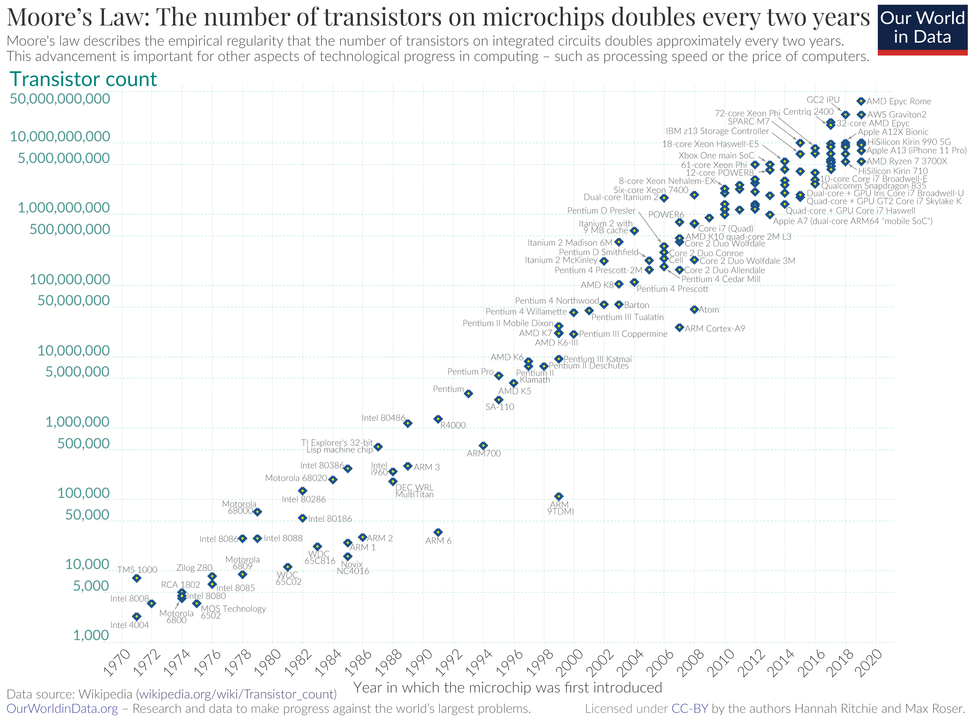
\includegraphics[scale=0.35]{moore.png}
\end{center}
\caption{Murov zakon}
\label{fig:frog}
\end{figure}

Eksponencijalni napredak predložen u Murovom zakonu se koristi kao jedan od glavnih pokazatelja da rezumno očekivati dolazak singularnosti u skorijoj budućnosti.

Rej Kurcvail (eng.~{\em Jeff Hawkins}) predlaže zakon o ubrzanom povratku, generalizujuću Murov zakon na celokupnu tehnologiju i govori o tome da se brzina tehnološkog razvoja eksponencijalno povećava. Taj zakon primenjuje i na tehnologije kao što su materijalna, medicinska i druge. \cite{mog-6}

Kurcvail takođe veruje da će se singularnost desiti do 2045. godine, jer smatra da će tada veštačka inteligencija nadjačati ukupnu sumu moždanog kapaciteta celog čovečanstva. \cite{mog-6}


\subsection{Razvoj algoritama}

Neke tehnologije, kao 'seed AI' \cite{mog-7}, imaju potencijal da se ne samo ubrzaju, već i da poboljšaju svoju efikasnost promenom sopstvenog izvornog koda. 
Ovaj mehanizam se od čistog povećanja brzine izvršavanja razlikuje u dva pogleda.

Prvo, za njega nije potreban spoljni uticaj. Za razliku od hardverskog ubrzavanja, gde je potreban bar neki nivo interakcije od strane čoveka, u ovom mehanizmu AI sam menja sopstveni kod.

Drugo, kao po Vernor Vindžovom (eng.~{\em Vernor Vinge}) viđenju singularnosti, ovaj pristup može biti vrlo nepredvidiv. \cite{mog-8}

\subsection{Kritike}

Neki kritičari, kao Hjubert Drejfus (eng.~{\em Hubert Dreyfus}) tvrde da računari i mašine ne mogu dostići nivo ljudske inteligencije, dok neki kao fizičar Stiven Hoking {\em Stephen Hawking}) tvrde da je definicija inteligencije zanemarljiva ukoliko je krajnji rezultat isti. \cite{mog-9}

Martin Ford u svojoj knjzi "The Lights in the Tunnel: Automation, Accelerating Technology and the Economy of the Future" predlaže "tehnološki paradoks", gde tvrdi da do singularnosti neće doći, zato što bi ona dovela do masovne nezaposlenosti i smanjene trgovinske potražnje, jer bi se pokazala efikasnijom od radnika, što bi za uzvrat dovelo do smanjene inicijative da se ulaže u iste tehnologije. \cite{mog-10}



\section{Slike i tabele}
\label{slike_i_tabele}

Slike i tabele treba da budu u svom okruženju, sa odgovarajućim naslovima, obeležene labelom da koje omogućava referenciranje. 

\begin{primer} Ovako se ubacuje slika. Obratiti pažnju da je dodato i 
\begin{verbatim}
\usepackage{graphicx}
\end{verbatim}

\begin{figure}[h!]
\begin{center}
\includegraphics[scale=0.25]{frog.jpg}
\end{center}
\caption{Frog}
\label{fig:frog}
\end{figure}

Na svaku sliku neophodno je referisati se negde u tekstu. Na primer, na slici \ref{fig:frog} prikazane su pande. 
\end{primer}

\begin{primer} I tabele treba da budu u svom okruženju, i na njih je neophodno referisati se u tekstu. Na primer, u tabeli \ref{tab:tabela1} su prikazana različita poravnanja u tabelama.

\begin{table}[h!]
\begin{center}
\caption{Razlčita poravnanja u okviru iste tabele ne treba koristiti jer su nepregledna.}
\begin{tabular}{|c|l|r|} \hline
centralno poravnanje& levo poravnanje& desno poravnanje\\ \hline
a &b&c\\ \hline
d &e&f\\ \hline
\end{tabular}
\label{tab:tabela1}
\end{center}
\end{table}

\end{primer}





\section{Prvi naslov}
\label{sec:naslov1}


Ovde pišem tekst. 
Ovde pišem tekst. 
Ovde pišem tekst. 
Ovde pišem tekst. 
Ovde pišem tekst. 
Ovde pišem tekst. 
Ovde pišem tekst. 
Ovde pišem tekst. 


\subsection{Prvi podnaslov}
\label{subsec:podnaslov1}

Ovde pišem tekst. 
Ovde pišem tekst. 
Ovde pišem tekst. 
Ovde pišem tekst. 
Ovde pišem tekst. 
Ovde pišem tekst. 
Ovde pišem tekst. 

\subsection{Drugi podnaslov}
\label{subsec:podnaslov2}

Ovde pišem tekst. 
Ovde pišem tekst. 
Ovde pišem tekst. 
Ovde pišem tekst. 
Ovde pišem tekst. 
Ovde pišem tekst. 

\section{Drugi naslov}
\label{sec:naslov2}

Ovde pišem tekst. 
Ovde pišem tekst. 
Ovde pišem tekst. 
Ovde pišem tekst. 

\subsection{... podnaslov}
\label{subsec:podnaslovN}

Ovde pišem tekst. 
Ovde pišem tekst. 
Ovde pišem tekst. 
Ovde pišem tekst. 
Ovde pišem tekst. 
Ovde pišem tekst. 

\section{n-ti naslov}
\label{sec:naslovN}

Ovde pišem tekst. 
Ovde pišem tekst. 
Ovde pišem tekst. 
Ovde pišem tekst. 
Ovde pišem tekst. 

\subsection{... podnaslov}
\label{subsec:podnaslovK}

Ovde pišem tekst. 
Ovde pišem tekst. 
Ovde pišem tekst. 
Ovde pišem tekst. 
Ovde pišem tekst. 

\subsection{... podnaslov}
\label{subsec:podnaslovM}

Ovde pišem tekst. 
Ovde pišem tekst. 
Ovde pišem tekst. 
Ovde pišem tekst. 
Ovde pišem tekst. 

\section{Poslednji naslov}
\label{sec:naslovM}

Ovde pišem tekst. 
Ovde pišem tekst. 
Ovde pišem tekst. 
Ovde pišem tekst. 
Ovde pišem tekst. 
Ovde pišem tekst. 
Ovde pišem tekst. 
Ovde pišem tekst. 
Ovde pišem tekst. 

\section{Zaključak}
\label{sec:zakljucak}

Ovde pišem zaključak. 
Ovde pišem zaključak. 
Ovde pišem zaključak. 
Ovde pišem zaključak. 
Ovde pišem zaključak. 
Ovde pišem zaključak. 
Ovde pišem zaključak. 
Ovde pišem zaključak. 
Ovde pišem zaključak. 
Ovde pišem zaključak. 
Ovde pišem zaključak. 
Ovde pišem zaključak. 


\addcontentsline{toc}{section}{Literatura}
\appendix

\iffalse
\bibliography{seminarski} 
\bibliographystyle{plain}
\fi

\begin{thebibliography}{9}

\bibitem{laski2009software} J. Laski and W. Stanley. \emph{Software Verification and Analysis}. Springer- Verlag, London, 2009.

\bibitem{gcc} Free Software Foundation. GNU gcc, 2013. on-line at: http://gcc. gnu.org/.

\bibitem{mog-1} "What is the Singularity? | Singularity Institute for Artificial Intelligence",  \href{https://web.archive.org/web/20110908014050/http://singinst.org/overview/whatisthesingularity/}{Singinst.org}.

\bibitem{mog-2} Hanson, Robin (1998). \href{https://mason.gmu.edu/~rhanson/vc.html#hanson}{"Some Skepticism"}.

\bibitem{mog-3} Grace, Katja; Salvatier, John; Dafoe, Allan; Zhang, Baobao; Evans, Owain (24 May 2017). "When Will AI Exceed Human Performance? Evidence from AI Experts"

\bibitem{mog-4} Eliezer Yudkowsky, 1996 "Staring into the Singularity"

\bibitem{mog-5} https://spectrum.ieee.org/tech-luminaries-address-singularity

\bibitem{mog-6} Ray Kurzweil, The Singularity Is Near, Penguin Group, 2005

\bibitem{mog-7} Yampolskiy, Roman V. "Analysis of types of self-improving software." Artificial General Intelligence. Springer International Publishing, 2015.

\bibitem{mog-8} Eliezer S. Yudkowsky. "Power of Intelligence"

\bibitem{mog-9} Dreyfus & Dreyfus 2000, p. xiv: 'The truth is that human intelligence can never be replaced with machine intelligence simply because we are not ourselves "thinking machines" in the sense in which that term is commonly understood.' Hawking (1998): 'Some people say that computers can never show true intelligence whatever that may be. But it seems to me that if very complicated chemical molecules can operate in humans to make them intelligent then equally complicated electronic circuits can also make computers act in an intelligent way. And if they are intelligent they can presumably design computers that have even greater complexity and intelligence.'

\bibitem{mog-10}
\href{https://www.nytimes.com/2011/03/05/science/05legal.html}{"Armies of Expensive Lawyers, Replaced by Cheaper Software"}.

\bibitem{haltingproblem} A. M. Turing. \emph{On Computable Numbers, with an application to the Entscheidungsproblem}. Proceedings of the London Mathematical Society, 2(42):230–265, 1936.


\end{thebibliography}


\appendix
\section{Dodatak}
Ovde pišem dodatne stvari, ukoliko za time ima potrebe.
Ovde pišem dodatne stvari, ukoliko za time ima potrebe.
Ovde pišem dodatne stvari, ukoliko za time ima potrebe.
Ovde pišem dodatne stvari, ukoliko za time ima potrebe.
Ovde pišem dodatne stvari, ukoliko za time ima potrebe.


\end{document}
